\chapter{刷怪机制}
执行刷怪的函数为 NPC.SpawnNPC()。

如果NPC.noSpawnCycle为true,那么这一帧不刷怪,把NPC.noSpawnCycle重置为false。

如果要刷怪的话,会对每个未死亡的玩家执行刷怪过程。在\wiki{史莱姆雨}进行时,会在其他刷怪之前插入史莱姆雨的刷怪。史莱姆雨的刷怪是额外刷怪,不会影响正常刷怪。如果有一个玩家成功进行了正常刷怪,那么跳过剩余玩家的刷怪。

\begin{remark}
每帧中,除史莱姆雨刷怪外,至多只会在一个玩家周围进行一次成功刷怪。
\end{remark}

进行正常刷怪时,首先要判断刷怪率和刷怪量,然后决定是否要刷怪,然后决定刷怪点和刷怪面,最后决定刷什么怪。

\section{刷怪率和刷怪量}
刷怪率用于控制刷怪速度,刷怪量用于控制刷怪上限。

如果玩家的活跃敌怪数量达到了刷怪量,那么刷怪失败。活跃敌怪数量是以玩家为中心,宽为2activeRangeX,高为2activeRangeY的矩形中的NPC的加权和。不同NPC权重不同\footnote{ToDo:权重表}。

刷怪率为n,意味着每次判定时的基础刷怪概率为1/n。

刷怪率基础值为600,刷怪量基础值为5。接下来会按照下面步骤修改刷怪率和刷怪量。注意,列表中的各项不互斥:如果同时满足两项的条件,那么两项都要结算,结算顺序与描述顺序相同。
\begin{enumerate}
    \item 在困难模式中,刷怪率改为540,刷怪量改为6。
    \item 如果玩家纵坐标距离世界底端小于200格,刷怪量乘2。如果玩家纵坐标在rockLayer+sHeight之下且距离世界底端不小于200格,刷怪率乘0.4向下取整,刷怪量乘1.9向下取整。如果玩家纵坐标不在rockLayer+sHeight之下且在worldSurface+sHeight之下,刷怪率乘0.5(困难模式为0.45)向下取整,刷怪量乘1.7(困难模式为1.8)向下取整。如果玩家纵坐标不在worldSurface+sHeight之下:\begin{itemize}
        \item 如果在晚上,刷怪率乘0.6向下取整,刷怪量乘1.3向下取整。
        \item 如果在血月,刷怪率乘0.3向下取整,刷怪量乘1.8向下取整。该效果会与晚上叠加。
        \item 如果在南瓜月或霜月,并且玩家纵坐标在worldSurface之上,那么刷怪率乘0.2向下取整,刷怪量乘2。
        \item 如果在日食,刷怪率乘0.2向下取整,刷怪量乘1.9向下取整。
    \end{itemize}
    \item 如果在苔原环境,并且玩家纵坐标在worldSurface之上,刷怪量乘(1+Main.cloudAlpha)并向下取整,刷怪率乘(1-Main.cloudAlpha/2)并向下取整。
    \item 如果在地牢环境,刷怪率乘0.4向下取整,刷怪量乘1.7向下取整。如果不在地牢环境并且在沙尘暴环境,刷怪率乘0.9(困难模式为0.4)向下取整,刷怪量乘1.2(困难模式为1.5)向下取整。如果不在沙尘暴环境并且在地下沙漠环境,刷怪率乘0.3(困难模式为0.2)向下取整,刷怪量乘2。如果不在以上三种环境并且在丛林环境,刷怪率乘0.4向下取整,刷怪量乘1.5向下取整。如果不在以上四种环境并且在腐化或血腥环境,刷怪率乘0.65向下取整,刷怪量乘1.3向下取整。如果不在以上六种环境并且在陨石环境,刷怪率乘0.4向下取整,刷怪量乘1.1向下取整。
    \item 如果在神圣环境,并且玩家纵坐标在rockLayer+sHeight之下,刷怪率乘0.65向下取整,刷怪量乘1.3向下取整。
    \item 如果世界中有血肉墙并且玩家纵坐标距离世界底端小于200格,刷怪率乘3,刷怪量乘0.3向下取整。
    \item 如果玩家的活跃敌怪数量小于刷怪量的1/5,刷怪率乘0.6向下取整。如果玩家的活跃敌怪数量不小于刷怪量的1/5但是小于刷怪量的2/5,刷怪率乘0.7向下取整。如果玩家的活跃敌怪数量不小于刷怪量的2/5但是小于刷怪量的3/5,刷怪率乘0.8向下取整。如果玩家的活跃敌怪数量不小于刷怪量的3/5但是小于刷怪量的4/5,刷怪率乘0.9向下取整。
    \item 如果玩家纵坐标在worldSurface与rockLayer的中点之下,或者玩家在腐化或血腥环境:\begin{itemize}
        \item 如果玩家的活跃敌怪数量小于刷怪量的1/5,刷怪率乘0.7向下取整。
        \item 如果玩家的活跃敌怪数量不小于刷怪量的1/5但是小于刷怪量的2/5,刷怪率乘0.9向下取整。
    \end{itemize}
    \item 如果玩家有镇静药剂buff,刷怪率乘1.3向下取整,刷怪量乘0.7向下取整。如果玩家有向日葵buff,刷怪率乘1.2向下取整,刷怪量乘0.8向下取整。如果玩家有战斗药水buff,刷怪率乘0.5向下取整,刷怪量乘2。如果玩家有水蜡烛buff并且没有和平蜡烛buff,刷怪率乘0.75向下取整,刷怪量乘1.5向下取整。如果玩家有和平蜡烛buff,刷怪率乘1.3向下取整,刷怪量乘0.7向下取整。如果玩家在水蜡烛区域内,并且在太空,刷怪率乘0.5向下取整。
    \item 如果刷怪率低于60,重置为60。如果刷怪量高于15,重置为15。在南瓜月/霜月中(要求玩家纵坐标在worldSurface之上),刷怪率为20,刷怪量为5*(2+玩家数量)。在撒旦军团事件中,刷怪率为600,刷怪量为5。判定为事件刷怪,刷怪率为20,刷怪量为5*(2+玩家数量)。在骷髅王前的地牢环境,刷怪率为10。
    \item 如果判定为小动物刷怪:\begin{itemize}
        \item 如果玩家中心距离世界底端小于200格,刷怪量乘0.5向下取整。
        \item 如果玩家中心距离世界底端不小于200格,刷怪量乘0.6向下取整。
    \end{itemize}
    \item 未判定为事件刷怪,并且不在血月、南瓜月、霜月、日食、地牢环境、腐化环境、血腥环境、陨石环境、撒旦军团事件中,并且未判定为小动物刷怪,考虑玩家的活跃城镇NPC数量\footnote{活跃城镇NPC数量是以玩家为中心,宽为2sWidth,高为2sHeight的矩形内城镇NPC的加权和}与玩家中心到世界底端的距离:\\
    \begin{tabular}{|c|c|c|}
        \hline
        &距离小于200格&距离不小于200格\\\hline
        1个活跃城镇NPC&刷怪率乘1.25向下取整&刷怪率乘2向下取整\\\hline
        2个活跃城镇NPC&刷怪率乘1.5向下取整&刷怪率乘3向下取整\\\hline
        $\ge$3个活跃城镇NPC&刷怪率乘2&刷怪量乘0.6向下取整\\\hline
    \end{tabular}
\end{enumerate}

\section{刷怪点和刷怪面}
在通过了$\frac{1}{\textrm{刷怪率}}$的基础刷怪概率后,会选取刷怪位置。刷怪位置的选取有一定随机性,如果选取失败就重新选取,直到选取成功为止。如果选了50次还没有成功,这次刷怪就取消。选取刷怪位置的过程中,首先要选取一个刷怪点,然后根据刷怪点计算出刷怪面,刷怪位置就在刷怪面上面1格。

刷怪点是在一个矩形范围内随机选取的,这个矩形中图格的横坐标从玩家横坐标-生成区域宽度取到玩家横坐标+生成区域宽度,纵坐标从玩家纵坐标-生成区域高度取到玩家纵坐标+生成区域高度。如果矩形范围超出了世界边界,那么按照世界边界对矩形进行裁剪。

如果刷怪点处有未虚化的实体块,或者刷怪点处有人工背景墙,本次选取失败。

进行\hyperref[app22]{太空刷怪判定}。如果通过了太空刷怪判定,刷怪面就是刷怪点。如果未通过太空刷怪判定,从刷怪点向下搜索到第一个未虚化的实体块作为刷怪面;如果刷怪面在安全区域内,本次选取失败。

如果刷怪面上方3格$\times$3格区域有部分超出了世界边界,或者其内部有未虚化的实体块或熔岩,本次选取失败。

\section{刷怪类型}

\subsection{事件刷怪}
\begin{itemize}
    \item 玩家纵坐标在worldSurface+sHeight之上,玩家距离事件中心的横坐标距离小于3000像素,那么判定为事件刷怪。
    \item 玩家纵坐标在worldSurface+sHeight之上,事件中心到世界中心的横坐标距离不超过5格,玩家到n个城镇NPC的最近横坐标距离小于3000像素,那么有$1-(2/3)^n$的概率判定为事件刷怪。
    \item 玩家在四柱区域内,判定为事件刷怪。
\end{itemize}

\subsection{禁止穿墙刷怪}
\begin{itemize}
    \item 未判定为事件刷怪,玩家不在血月、南瓜月、霜月、日食、地牢环境、腐化环境、血腥环境、陨石环境、撒旦军团事件中,玩家中心距离世界底端不小于200格,判定禁止穿墙刷怪。
    \item 未判定为事件刷怪,玩家不在血月、南瓜月、霜月、日食、地牢环境、腐化环境、血腥环境、陨石环境、撒旦军团事件中,玩家中心距离世界底端小于200格,对应于玩家的活跃城镇NPC数量,分别有1/2概率(1个活跃城镇NPC)、3/4概率(2个活跃城镇NPC)、9/10概率($\ge$3个活跃城镇NPC)判定禁止穿墙刷怪。
    \item 玩家中心在人工背景墙前,判定禁止穿墙刷怪。
\end{itemize}

\subsection{小动物刷怪}
未判定为事件刷怪,并且不在血月、南瓜月、霜月、日食、地牢环境、腐化环境、血腥环境、陨石环境、撒旦军团事件中,玩家的活跃城镇NPC数量与玩家中心到世界底端的距离会决定小动物刷怪的概率:\\
\begin{center}
\begin{tabular}{|c|c|c|}
    \hline
    &距离小于200格&距离不小于200格\\\hline
    1个活跃城镇NPC&1/10&1/3\\\hline
    2个活跃城镇NPC&1/5&1/2\\\hline
    $\ge$3个活跃城镇NPC&1/3&专家模式29/30,普通模式一定\\\hline
\end{tabular}
\end{center}

\subsection{太空刷怪}\label{app22}
太空刷怪是在刷怪面选取过程中判定的。太空刷怪的前提是未判定为事件刷怪且未判定为小动物刷怪。
\begin{itemize}
    \item 如果刷怪点纵坐标在0.35worldSurface之上,并且是困难模式,判定为太空刷怪。
    \item 如果刷怪点纵坐标在0.35worldSurface之上,并且刷怪点到世界中心的水平距离大于世界宽度的0.05倍,判定为太空刷怪。
    \item 如果刷怪点纵坐标在0.45worldSurface之上,并且是困难模式,有1/10概率判定为太空刷怪。
\end{itemize}

\subsection{水中刷怪}
如果刷怪面上方的两格都有液体,并且刷怪面上方一格是水,判定为水中刷怪。

\subsection{大理石刷怪与花岗岩刷怪}
如果刷怪面是大理石块,判定为大理石刷怪。如果刷怪面是花岗岩块,判定为花岗岩刷怪。刷怪面既不是大理石块也不是花岗岩块,再看玩家脚下的图格\footnote{具体为玩家脚下8像素处的图格};如果这一格为大理石块,判定为大理石刷怪;如果这一格为花岗岩块,判定为花岗岩刷怪。

如果以上条件均未满足,判定较复杂。如果读者看不懂\autoref{algo1},只用记住,玩家附近和刷怪面附近大理石/花岗岩越多,越容易刷对应怪。进入到这一级判定时,可以同时判定为刷大理石怪和花岗岩怪。

\begin{algorithm}[!h]
\caption{大理石/花岗岩刷怪判定算法}\label{algo1}
\SetKwInOut{KIN}{输入}
\SetKwInOut{KOUT}{输出}
\SetKw{IN}{in}
\SetArgSty{textrm}
\KIN{刷怪面坐标(x1,y1),玩家脚下图格坐标(x2,y2)}
\KOUT{大理石刷怪判定flag1,花岗岩刷怪判定flag2}
flag1=flag2=false\;
size1是20到30的随机整数\; 
stepX1是1到3的随机整数; stepY1是1到3的随机整数\;
\lIf{x1-size1<0}{size1=x1}
\lIf{y1-size1<0}{size1=y1}
\lIf{x1+size1>=maxTileX}{size1=maxTileX-x1-1}
\lIf{y1+size1>=maxTileY}{size1=maxTileY-y1-1}
\For{x \IN x1-size1:stepX1:x1+size1}{
    \For{y \IN y1-size1:stepY1:y1+size1}{
        如果(x,y)处的图格为大理石,flag1=true\;
        如果(x,y)处的图格为花岗岩,flag2=true\;
    }
}
size2是30到60的随机整数\; 
stepX2是3到6的随机整数; stepY2是3到6的随机整数\;
\lIf{x2-size2<0}{size2=x2}
\lIf{y2-size2<0}{size2=y2}
\lIf{x2+size2>=maxTileX}{size2=maxTileX-x2-2}
\lIf{y2+size2>=maxTileY}{size2=maxTileY-y2-2}
\For{x \IN x2-size2:stepX2:x2+size2}{
    \For{y \IN y2-size2:stepY2:y2+size2}{
        如果(x,y)处的图格为大理石,flag1=true\;
        如果(x,y)处的图格为花岗岩,flag2=true\;
    }
}
\end{algorithm}

\subsection{蜘蛛巢刷怪和地下沙漠刷怪}
蜘蛛巢刷怪和地下沙漠刷怪都是通过背景墙判定的。蜘蛛巢刷怪通过蜘蛛墙判定,地下沙漠刷怪通过沙岩墙、硬化沙墙和它们的三化对应墙判定。这两个刷怪是独立判定的,可以同时判定为蜘蛛巢刷怪和地下沙漠刷怪。

这两个刷怪的前提是玩家不在地牢环境,未判定为事件刷怪。蜘蛛巢刷怪要求刷怪面在rockLayer之下,刷怪面距离世界底端大于200格。地下沙漠刷怪要求刷怪面在rockLayer之上,刷怪面距离世界顶端大于200格。

有1/3概率通过刷怪面附近区域内背景墙判定。以刷怪面为中心,取一个正方形区域,其边长是11到29的一个奇数格。如果这个正方形区域没有超出世界边界并且其中存在一个对应的墙,判定成功,否则判定失败。

在另外2/3概率中,直接通过玩家坐标所在格的背景墙判定。

\begin{remark}
即使玩家站在对应的背景墙前,如果刷怪面附近没有对应背景墙,仍有1/3概率判定失败。
\end{remark}

\section{刷怪失败}
前面已经说过,选取失败后还会再次选取,一共有50次机会。如果50次都没有成功,那么本次刷怪失败。

如果玩家的活跃敌怪数量达到了刷怪量,刷怪失败。

如果刷怪面碰撞箱与以某个玩家为中心,宽sWidth+2safeRangeX,高sHeight+2safeRangeY的矩形相交,本次刷怪失败。

如果在地牢环境,但是刷怪面不是地牢方块或者刷怪面上方一格没有背景墙,本次刷怪失败。

如果刷怪面上方两格都是液体,并且刷怪面上方一格是蜂蜜,刷怪失败。

\section{刷怪种类}
刷怪的优先级是四柱>太空>事件>昏迷男子>蜘蛛巢>地下沙漠>巨骨舌鱼>血水母>嗜血怪>海洋>沉睡渔夫>食人鱼>蓝水母>水中小动物>受缚哥布林>受缚巫师>小动物>地牢>陨石>撒旦军团>霜月>南瓜月>日食>发光蘑菇地>腐地蠕虫>宝箱怪>幻灵>弹跳杰克南瓜灯>骷髅博士>紫胶虫>地下蠕虫>老鼠>蜗牛>丛林青蛙>困难模式丛林>丛林>沙尘暴>木乃伊>地表神圣>附魔剑>猩红之地>腐化之地>地表综合>地表白天>地表夜晚>地下>地狱>洞穴。

每级的名称不唯一对应某些怪,有些怪会同时出现在多级中。

所有判定完成后,如果新生成的怪是蓝史莱姆,有1/180概率被替换为粉史莱姆(ID:-4)。

\subsection{四柱}
如果玩家在四柱附近,那么就会刷四柱怪。四柱刷怪的优先级是\wiki{星云柱}>\wiki{星旋柱}>\wiki{星尘柱}>\wiki{日曜柱}。

\subsubsection{星云柱}
刷怪为\wiki{星云浮怪}、\wiki{吮脑怪}、\wiki{进化兽}、\wiki{预言帝}。这四个怪的刷怪比例为1:5:3:3。星云浮怪在整个世界中的上限为2个,进化兽在整个世界中的上限为3个,预言帝在整个世界中的上限为2个。这个刷怪比例\&上限的规则是四柱的特色。举例来说,没有任何刷怪的时候,这四个怪的刷怪概率分别是1/12、5/12、1/4、1/4;如果已经刷出了两个星云浮怪,那么不会再刷星云浮怪,剩下三个怪的刷怪概率分别是5/11、3/11、3/11。
\begin{figure}
    \centering
    \subfloat[星云浮怪]{\quad
\includegraphics{npcs/Nebula_Floater.png}\quad}
    \subfloat[吮脑怪]{\quad
\includegraphics{npcs/Brain_Suckler.png}\quad}
    \subfloat[进化兽]{\quad
\includegraphics{npcs/Evolution_Beast.png}\quad}
    \subfloat[预言帝]{\quad
\includegraphics{npcs/Predictor.png}\quad}
    \caption{星云柱}
\end{figure}

\subsubsection{星旋柱}
刷怪为\wiki{漩泥怪}、\wiki{异星蜂王}、\wiki{异星黄蜂}、\wiki{星旋怪}。刷怪比例为2:1:2:4。漩泥怪上限为3,异星蜂王上限为3,星旋怪上限为4。
\begin{figure}
    \centering
    \subfloat[漩泥怪]{\quad
\includegraphics{npcs/Storm_Diver.png}\quad}
    \subfloat[异星蜂王]{\quad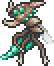
\includegraphics{npcs/Alien_Queen.png}\quad}
    \subfloat[异星黄蜂]{\quad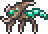
\includegraphics{npcs/Alien_Hornet.png}\quad}
    \subfloat[星旋怪]{\quad
\includegraphics{npcs/Vortexian.png}\quad}
    \caption{星旋柱}
\end{figure}

\subsubsection{星尘柱}
刷怪为\wiki{银河织妖}、\wiki{星细胞}、\wiki{流体入侵怪}、\wiki{闪耀炮手}、\wiki{观星怪}。刷怪比例为1:1:1:2:3。
\begin{figure}
    \centering
    \subfloat[银河织妖]{\quad
\includegraphics{npcs/Milkyway_Weaver.png}\quad}\\
    \subfloat[星细胞]{\quad
\includegraphics{npcs/Star_Cell.png}\quad}
    \subfloat[流体入侵怪]{\quad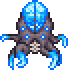
\includegraphics{npcs/Flow_Invader.png}\quad}
    \subfloat[闪耀炮手]{\quad
\includegraphics{npcs/Twinkle_Popper.png}\quad}
    \subfloat[观星怪]{\quad
\includegraphics{npcs/Stargazer.png}\quad}
    \caption{星尘柱}
\end{figure}

\subsubsection{日曜柱}
刷怪为\wiki{千足蜈蚣}、\wiki{火龙怪}、\wiki{火龙怪骑士}、\wiki{火滚怪}、\wiki{流星火怪}、\wiki{火月怪}、\wiki{火龙战士}。刷怪比例为1:1:1:1:1:1:1。千足蜈蚣上限为1,火龙怪上限为2,火龙怪骑士上限为1,火龙战士上限为2。
\begin{figure}
    \centering
    \subfloat[千足蜈蚣]{\quad
\includegraphics{npcs/300px-Crawltipede.png}\quad}\\
    \subfloat[火龙怪]{\quad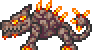
\includegraphics{npcs/Drakomire.png}\quad}
    \subfloat[火龙怪骑士]{\quad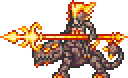
\includegraphics{npcs/Drakomire_Rider.png}\quad}
    \subfloat[火滚怪]{\quad
\includegraphics{npcs/Sroller.png}\quad}\\
    \subfloat[流星火怪]{\quad
\includegraphics{npcs/Corite.png}\quad}
    \subfloat[火月怪]{\quad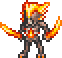
\includegraphics{npcs/Selenian.png}\quad}
    \subfloat[火龙战士]{\quad
\includegraphics{npcs/Drakanian.png}\quad}
    \caption{日曜柱}
\end{figure}

\subsection{太空刷怪}
优先级是火星飞船>火星探测器>飞龙>鸟妖。

如果执行的是火星入侵的刷怪,那么生成\wiki{火星飞船}。

在石巨人后,通过了Boss与事件检查,玩家中心在\hyperref[app9]{透光墙}或\wiki{云墙}前,刷怪面到世界中心的横坐标距离大于世界宽度$\times$0.165\footnote{小世界为693格,中世界为1056格,大世界为1386格},那么有概率生成\wiki{火星探测器},这个概率与是否打过火星入侵、是否在水蜡烛区域、是否有水蜡烛buff相关(\autoref{tab5651})。水蜡烛区域和水蜡烛buff不是一回事,水蜡烛区域不包括手持水蜡烛的情况。火星探测器的上限为1。

\begin{table}[!h]
    \centering
    \begin{tabular}{cccccc}
         000&001&011&100&101&111\\\hline
         1/8&15/64&5/9&1/30&59/900&19/100 
    \end{tabular}
    \caption{二进制的第一位表示是否打过火星入侵,第二位表示是否在水蜡烛区域,第三位表示是否有水蜡烛buff。例如101表示打过火星入侵,不在水蜡烛区域内,有水蜡烛buff。}
    \label{tab5651}
\end{table}

没有水蜡烛buff的时候,\wiki{飞龙}的生成概率为1/10;有水蜡烛buff的时候生成概率为19/100。飞龙的上限为1。当禁止穿墙刷怪时不会刷飞龙。

如果火星飞船、火星探测器、飞龙均未生成,那么生成鸟妖。
\begin{figure}
    \centering
    \subfloat[火星飞船]{\quad
\includegraphics{npcs/Martian_Drone.png}\quad}
    \subfloat[火星探测器]{\quad
\includegraphics{npcs/Martian_Probe.png}\quad}
    \subfloat[鸟妖]{\quad
\includegraphics{npcs/Harpy.png}\quad}\\
    \subfloat[飞龙]{\quad
\includegraphics{npcs/299px-Wyvern.png}\quad}
    \caption{太空刷怪}
\end{figure}

\subsection{事件刷怪}
\subsubsection{\wiki{哥布林入侵}}
1/9概率生成\wiki{哥布林巫士},8/45概率生成\wiki{哥布林苦力},32/135概率生成\wiki{哥布林弓箭手},32/405概率生成\wiki{哥布林盗贼},64/405概率生成\wiki{哥布林战士}。在困难模式中,有1/30概率生成\wiki{哥布林召唤师},这会覆盖前面的生成。哥布林召唤师上限为1。
\begin{figure}
    \centering
    \subfloat[哥布林巫士]{\qquad
\includegraphics{npcs/Goblin_Sorcerer.png}\qquad}
    \subfloat[哥布林苦力]{\qquad
\includegraphics{npcs/Goblin_Peon.png}\qquad}
    \subfloat[哥布林弓箭手]{\qquad
\includegraphics{npcs/Goblin_Archer.png}\qquad}
    \subfloat[哥布林盗贼]{\qquad
\includegraphics{npcs/Goblin_Thief.png}\qquad}
    \subfloat[哥布林战士]{\qquad
\includegraphics{npcs/Goblin_Warrior.png}\qquad}
    \subfloat[哥布林召唤师]{\qquad
\includegraphics{npcs/Goblin_Summoner.png}\qquad}
    \caption{哥布林入侵}
\end{figure}

\subsubsection{\wiki{雪人入侵}}
1/7概率生成\wiki{巴拉雪人},2/7概率生成\wiki{雪人暴徒};4/7概率生成\wiki{戳刺先生}。
\begin{figure}
    \centering
    \subfloat[巴拉雪人]{\quad
\includegraphics{npcs/Snow_Balla.png}\quad}
    \subfloat[雪人暴徒]{\quad
\includegraphics{npcs/Snowman_Gangsta.png}\quad}
    \subfloat[戳刺先生]{\quad
\includegraphics{npcs/Mister_Stabby.png}\quad}
    \caption{雪人入侵}
\end{figure}

\subsubsection{\wiki{海盗入侵}}
1/11概率生成\wiki{海盗弩手},10/99概率生成\wiki{鹦鹉},80/693概率生成\wiki{海盗神射手},160/693概率生成\wiki{私船海盗},320/693概率生成\wiki{海盗水手}。

\wiki{海盗船长}有1/30概率生成,会覆盖前面的生成。海盗船长上限为1。

\wiki{荷兰飞盗船}生成要求入侵进度超过一半,并且刷怪面的左右各20格,上方10格到40格范围内没有实体块。荷兰飞盗船生成概率是1/20。荷兰飞盗船上限为1。荷兰飞盗船的生成会覆盖其他生成。
\begin{figure}
    \centering
    \subfloat[海盗弩手]{\quad
\includegraphics{npcs/Pirate_Crossbower.png}\quad}
    \subfloat[鹦鹉]{\quad
\includegraphics{npcs/Parrot.png}\quad}
    \subfloat[海盗神射手]{\quad
\includegraphics{npcs/Pirate_Deadeye.png}\quad}
    \subfloat[私船海盗]{\quad
\includegraphics{npcs/Pirate_Corsair.png}\quad}
    \subfloat[海盗水手]{\quad
\includegraphics{npcs/Pirate_Deckhand.png}\quad}
    \subfloat[海盗船长]{\quad
\includegraphics{npcs/Pirate_Captain.png}\quad}\\
    \subfloat[荷兰飞盗船]{\quad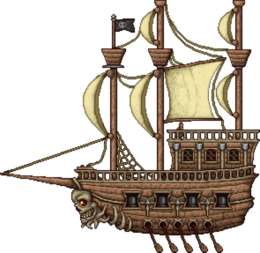
\includegraphics{npcs/260px-Flying_Dutchman.png}\quad}
    \caption{海盗入侵}
\end{figure}

\subsubsection{\wiki{火星入侵}}
\wiki{火星飞碟}的生成分为两段判定。离入侵结束不到100分\footnote{入侵事件总分为160+40$\times$玩家数量}时,火星飞碟的概率为1/10并且会覆盖其他生成(包括第二段)。第二段中火星飞碟和其他敌怪处理方法相同。

火星飞碟上限为1,\wiki{火星走妖}上限为1。以下是第二段判定。

火星飞碟概率为1/70,\wiki{鳞甲怪}和\wiki{火星工程师}概率均为9/140(火星飞碟达到上限的话,这个概率变为1/14),\wiki{火星飞船}概率为2/35,\wiki{扰脑怪}概率为4/35,\wiki{激光枪手}概率为4/35,\wiki{火星走妖}概率为1/7,\wiki{灰咕噜兽}、\wiki{电击怪}和\wiki{火星军官}概率均为1/7(火星走妖达到上限的话,这个概率为4/21)。
\begin{figure}
    \centering
    \subfloat[火星飞碟]{\quad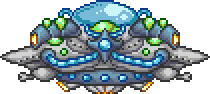
\includegraphics{npcs/Martian_Saucer.png}\quad}
    \subfloat[火星走妖]{
\includegraphics{npcs/Martian_Walker.png}}
    \subfloat[鳞甲怪]{\quad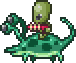
\includegraphics{npcs/Scutlix.png}\quad}\\
    \subfloat[火星工程师]{\qquad
\includegraphics{npcs/Martian_Engineer.png}\qquad}
    \subfloat[火星飞船]{
\includegraphics{npcs/Martian_Drone.png}}
    \subfloat[扰脑怪]{\quad
\includegraphics{npcs/Brain_Scrambler.png}\quad}
    \subfloat[激光枪手]{\qquad
\includegraphics{npcs/Ray_Gunner.png}\qquad}
    \subfloat[灰咕噜兽]{\qquad
\includegraphics{npcs/Gray_Grunt.png}\qquad}
    \subfloat[电击怪]{\quad
\includegraphics{npcs/Gigazapper.png}\quad}
    \subfloat[火星军官]{\quad
\includegraphics{npcs/Martian_Officer.png}\quad}
    \caption{海盗入侵}
\end{figure}

\subsection{\wiki{昏迷男子}}
满足昏迷男子生成条件,并且不是水中刷怪,那么有1/80概率生成昏迷男子。

\subsection{\wiki{蜘蛛巢}}
刷怪面有蜘蛛墙,不高于 rockLayer,距离世界底端大于210格,且不是水中刷怪,未解救过\wiki{发型师},那么有1/8概率生成\wiki{受缚发型师}。

在未生成受缚发型师的前提下,如果刷怪面有蜘蛛墙或者判定为蜘蛛巢刷怪,那么困难模式生成\wiki{黑隐士},困难模式前生成\wiki{爬墙蜘蛛}。

\subsection{\wiki{地下沙漠}}
进行地下沙漠刷怪的要求是判定为地下沙漠刷怪,刷怪面在地下,并且刷怪面上的背景墙是硬化沙墙/沙岩墙,或者它们的转化墙\footnote{神圣化、腐化、血腥化}。刷怪优先级是沙虫>墓穴爬虫>困难模式>其他。

\wiki{沙虫}和\wiki{墓穴爬虫}的生成都要求不禁止穿墙刷怪,并且刷怪面在地表下100格以下。沙虫的概率为1/33,墓穴爬虫的概率为1/22。沙虫只会在困难模式生成。

在困难模式中,有4/5的概率进行困难模式刷怪。困难模式的刷怪有\wiki{腐恶食尸鬼}、\wiki{红染食尸鬼}、\wiki{神梦食尸鬼}、\wiki{食尸鬼}、\wiki{沙漠幽魂}、\wiki{邪恶拉弥亚}、\wiki{沙贼}、\wiki{拉弥亚}、\wiki{蛇蜥怪},它们的刷怪比例为2:2:2:2:1:1:1:1:1,\wiki{腐恶食尸鬼}在腐化环境生成,\wiki{红染食尸鬼}在血腥环境生成,\wiki{神梦食尸鬼}在神圣环境生成,\wiki{食尸鬼}只在纯净环境生成,\wiki{沙漠幽魂}和\wiki{邪恶拉弥亚}在腐化或血腥环境生成,\wiki{沙贼}和\wiki{拉弥亚}在没有腐化和血腥的环境生成,\wiki{蛇蜥怪}不挑环境。举例来说,如果玩家同时处在血腥和神圣环境中,那么可以生成\wiki{红染食尸鬼}、\wiki{神梦食尸鬼}、\wiki{沙漠幽魂}、\wiki{邪恶拉弥亚}、\wiki{蛇蜥怪},其刷怪比例为2:2:1:1:1。

既没刷出沙虫或墓穴爬虫,也没有困难模式刷怪,那么刷\wiki{蚁狮}/\wiki{蚁狮马}/\wiki{蚁狮蜂},刷怪比例为1:3:1。

\subsection{\wiki{巨骨舌鱼}}
困难模式+水中刷怪+丛林环境,2/3概率生成巨骨舌鱼。

\subsection{\wiki{血水母}}
困难模式+水中刷怪+血腥环境,2/3概率生成血水母。

\subsection{\wiki{嗜血怪}}
困难模式+水中刷怪+血腥环境,2/3概率生成嗜血怪。

\subsection{\wiki{海洋}}
要求:水中刷怪,刷怪横坐标距离地图左右边界<250格,刷怪面是沙块或珍珠/黑檀/猩红沙块,刷怪面纵坐标在rockLayer之上。优先级:沉睡渔夫>其他。

\subsubsection{\wiki{沉睡渔夫}}
要求:刷怪横坐标在安全区域外,满足沉睡渔夫生成条件。

从刷怪面向上搜索47格(不包括刷怪面)找到第一个可以生成沉睡渔夫的图格,这一格需要满足:没有实体块;上方第一格没有实体块;上方第二格没有液体;上方第二格没有实体块。如果找到了这一格,那么生成沉睡渔夫。

\subsubsection{其他}
1/60概率生成\wiki{海蜗牛},59/1500概率生成\wiki{乌贼},59/500概率生成\wiki{鲨鱼},413/1500概率生成\wiki{螃蟹},413/750概率生成\wiki{粉水母}。

\subsection{沉睡渔夫}
要求:不是水中刷怪,刷怪横坐标距离地图左右边界<340格,刷怪面是沙块或珍珠/黑檀/猩红沙块刷怪面纵坐标在worldSurface之上,满足沉睡渔夫生成条件。生成沉睡渔夫。

\subsection{\wiki{食人鱼}}
要求:水中刷怪。刷怪面在rockLayer之下,有1/2概率生成食人鱼;刷怪面是丛林草皮,必然生成食人鱼。在困难模式,生成的食人鱼有2/3概率转化为\wiki{琵琶鱼}。

\subsection{\wiki{蓝水母}}
要求:水中刷怪,刷怪面在worldSurface之下。有1/3概率生成蓝水母。困难模式中生成的蓝水母转化为\wiki{绿水母}。

\subsection{水中小动物}
如果是水中刷怪,在腐化环境有1/4概率生成\wiki{腐化金鱼}。

如果是水中刷怪,不在腐化环境,刷怪面在worldSurface之上,刷怪面距离世界顶端大于50格,在白天,有1/6概率在水面\footnote{这里的水面判定与海洋沉睡渔夫的判定相同。}等概率生成\wiki{鸭}或\wiki{野鸭}。上一句话中没有成功生成的话,生成\wiki{金鱼}。

如果未判定生成小动物,那么生成友好水中小动物的概率额外乘1/4。

\subsection{\wiki{受缚哥布林}}
要求:满足受缚哥布林生成条件,不是水中刷怪,刷怪面不在rockLayer之上,刷怪面距离世界底端大于210格。有1/20概率生成受缚哥布林。

\subsection{\wiki{受缚巫师}}
要求:满足受缚巫师生成条件,,不是水中刷怪,刷怪面不在rockLayer之上,刷怪面距离世界底端大于210格。有1/20概率生成受缚巫师。

\subsection{\wiki{小动物}}
要求:判定生成小动物,不是水中刷怪。丛林草皮上有1/150概率生成\wiki{金蛙},149/150概率生成\wiki{青蛙}。雪块和冰雪块上\wiki{企鹅}和\wiki{蓝企鹅}生成概率各半。在草皮或神圣草皮上的刷怪优先级:雨天>萤火虫>鸟(1)>蝴蝶>鸟(2)>兔兔和松鼠。其他情况下,如果刷怪面不在worldSurface之下,生成失败;否则生成规则与草皮上的生成规则相同,除了在刷怪面是沙块时,兔兔和松鼠会被各1/2概率生成的\wiki{黑蝎子}和\wiki{蝎子}替代。

\subsubsection{\wiki{雨天}}
在雨天,2/3概率生成\wiki{蠕虫},1/3概率生成\wiki{步行金鱼}。此外,有1/150的概率它们会被\wiki{金蠕虫}覆盖。

\subsubsection{\wiki{萤火虫}}\label{app14}
要求:在晚上,刷怪面不在worldSurface之下。如果刷怪面是草皮,生成萤火虫;否则生成\wiki{荧光虫}。有1/fireFlyFriendly的概率生成。在成功生成的前提下,在刷怪面的上下左右共4格分别有1/fireFlyMultiple的概率额外生成一个。

有1/9的概率,fireFlyFriendly在1到3随机,fireFlyMultiple在3到7随机;有8/27的概率,fireFlyFriendly和fireFlyMultiple均为999999;有16/27的概率,fireFlyFriendly在2到14随机,fireFlyMultiple在6到29随机。它们的值在每天入夜时刷新。

\subsubsection{鸟(1)}\label{app13}
要求:在4:30到9:30,刷怪面不在worldSurface之下。有2/3概率生成某种鸟。

在确定生成某种鸟的前提下,有1/4概率生成\wiki{红雀},1/4概率生成\wiki{冠蓝鸦},1/2概率生成\wiki{鸟}.此外,有1/150的概率它们会被\wiki{金鸟}覆盖。

\subsubsection{蝴蝶}\label{app11}
要求:白天,刷怪面不在worldSurface之下。生成某种蝴蝶的概率是1/butterflyChance。butterflyChance的值在每天入夜时刷新,有1/3概率为999999,剩下2/3概率在1到24随机。

在确定生成某种蝴蝶的前提下,有1/150概率生成\wiki{金蝴蝶},149/150概率生成\wiki{蝴蝶}。此外,在刷怪面的左右共2格分别有1/4的概率额外生成一个蝴蝶。

\subsubsection{鸟(2)}
要求:刷怪面不在worldSurface之下。有1/2概率生成某种鸟。其他刷怪概率与鸟(1)相同。

\subsubsection{兔兔和松鼠}\label{app12}
各种松鼠要求刷怪面不在worldSurface之下。刷怪优先级:金兔>金松鼠>史莱姆兔兔>圣诞节兔兔>派对兔兔>松鼠=红松鼠>兔兔。\wiki{金兔}概率1/150,\wiki{金松鼠}概率1/150,\wiki{史莱姆兔兔}概率2/3(要求万圣节期间),\wiki{圣诞节兔兔}概率2/3(要求圣诞节期间),\wiki{派对兔兔}概率2/3(要求派对期间),\wiki{松鼠}和\wiki{红松鼠}概率各1/6,以上所有均未成功生成的,生成\wiki{兔兔}。

\subsection{\wiki{地牢}}
要求:在地牢环境。刷怪优先级:地牢守卫>受缚机械师>骷髅李小龙>骷髅突击手=骷髅狙击手=骷髅特警>圣骑士=巨型诅咒骷髅头>褴褛邪教徒法师=死灵法师=魔教徒>生锈装甲骷髅=蓝装甲骷髅=地狱装甲骷髅>地牢史莱姆>尖刺球=烈焰火轮=诅咒骷髅头>暗黑法师>愤怒骷髅怪。部分敌怪只会在击败世纪之花后的困难模式出现,而且部分敌怪的生成依赖于刷怪面的背景墙种类,这两个信息下文会省略。

如果没打过骷髅王,生成\wiki{地牢守卫}。未解救\wiki{机械师},刷怪面在rockLayer之下,有1/5概率生成\wiki{受缚机械师}。\wiki{骷髅李小龙}概率1/30。\wiki{骷髅突击手}、\wiki{骷髅狙击手}、\wiki{骷髅特警}概率都是1/15。\wiki{圣骑士}概率1/35,世界中只能存在一个。\wiki{巨型诅咒骷髅头}概率1/30。\wiki{褴褛邪教徒法师}、\wiki{死灵法师}、\wiki{魔教徒}概率都是1/20;它们各有两个ID,生成概率均等;世界中分别只能存在一个。\wiki{生锈装甲骷髅}、\wiki{蓝装甲骷髅}、\wiki{地狱装甲骷髅}概率都是2/3;它们各有4个ID,生成概率均等。\wiki{地牢史莱姆}概率1/37。\wiki{尖刺球}概率1/4;要求以刷怪面为中心的边长600像素的正方形与最近的另一个尖刺球的支撑块不相交。\wiki{烈焰火轮}概率1/15。\wiki{诅咒骷髅头}概率1/9。\wiki{暗黑法师}概率1/7。

以上均未生成时,生成\wiki{愤怒骷髅怪}。愤怒骷髅怪一共有6个ID:294、295、296、31、-14、-13,它们的概率分别是1/5、1/5、1/5、6/25、1/10、3/50。

\subsection{\wikii{陨石(生物群落)}{陨石}}
在陨石环境,生成\wiki{流星头}。

\subsection{撒旦军队}
\wiki{撒旦军队}事件在进行时,并且玩家在事件区域内,那么不刷怪。

\subsection{\wiki{霜月}}
要求:刷怪面不高于worldSurface,在晚上,在霜月中。刷怪优先级:礼物宝箱怪>其他。

与波数无关的是\wiki{礼物宝箱怪}。只要世界中只存在不到4个礼物宝箱怪,它就会以1/30的概率生成。

第20波,\wiki{冰雪女王}、\wiki{圣诞坦克}、\wiki{常绿尖叫怪}概率各1/3。

第19波,刷怪优先级:冰雪女王>圣诞坦克>常绿尖叫怪>雪兽。\wiki{冰雪女王}概率1/10,上限4个。\wiki{圣诞坦克}概率1/10,上限5个。\wiki{常绿尖叫怪}概率1/10,上限7个。这三个怪都不生成的情况下生成\wiki{雪兽}。

第18波,刷怪优先级:冰雪女王>圣诞坦克>常绿尖叫怪>其他。\wiki{冰雪女王}概率1/10,上限3个。\wiki{圣诞坦克}概率1/10,上限4个。\wiki{常绿尖叫怪}概率1/10,上限6个。这三个怪都不生成的情况下,\wiki{胡桃夹士}概率1/3,\wiki{坎卜斯}概率2/9,\wiki{雪兽}概率4/9。

第17波,刷怪优先级:冰雪女王>圣诞坦克>常绿尖叫怪>其他。冰雪女王概率1/10,上限2个。圣诞坦克概率1/10,上限3个。常绿尖叫怪概率1/10,上限5个。这三个怪都不生成的情况下,精灵直升机(ID:347)概率1/4,坎卜斯概率3/8,雪兽概率3/8。

第16波,刷怪优先级:冰雪女王>圣诞坦克>常绿尖叫怪>其他。冰雪女王概率1/10,上限2个。圣诞坦克概率1/10,上限2个。常绿尖叫怪概率1/10,上限4个。这三个怪都不生成的情况下,雪花怪(ID:352)概率1/2,雪兽概率1/2。

第15波,刷怪优先级:冰雪女王>圣诞坦克>常绿尖叫怪>其他。冰雪女王概率1/10,上限1个。圣诞坦克概率1/10,上限2个。常绿尖叫怪概率1/10,上限3个。这三个怪都不生成的情况下,精灵直升机概率1/3,雪兽概率2/3。

第14波,刷怪优先级:冰雪女王>圣诞坦克>常绿尖叫怪>其他。冰雪女王概率1/10,上限1个。圣诞坦克概率1/10,上限1个。常绿尖叫怪概率1/10,上限1个。这三个怪都不生成的情况下,雪兽概率1/3,不刷怪概率2/3。

第13波,刷怪优先级:冰雪女王>圣诞坦克>其他。冰雪女王概率1/10,上限1个。圣诞坦克概率1/10,上限1个。这两个怪都不生成的情况下,雪花怪概率1/3,雪兽概率1/9,姜饼人(ID:342)概率5/27,精灵直升机概率10/27。

第12波,刷怪优先级:冰雪女王>常绿尖叫怪>其他。冰雪女王概率1/10,上限1个。常绿尖叫怪概率1/10,上限1个。这两个怪都不生成的情况下,雪兽概率1/8,姜饼人概率7/24,僵尸精灵(ID:338/339/340)概率7/12。僵尸精灵的三个ID等概率生成。

第11波,刷怪优先级:冰雪女王>其他。冰雪女王概率1/10,上限1个。冰雪女王不生成的情况下,雪花怪概率1/6,姜饼人概率5/12,僵尸精灵概率5/12。

第10波,刷怪优先级:圣诞坦克>常绿尖叫怪>其他。圣诞坦克概率1/10,上限1个。常绿尖叫怪概率1/10,上限2个。这两个怪都不生成的情况下,坎卜斯概率1/6,胡桃夹士概率5/18,精灵直升机概率5/27,僵尸精灵概率10/27。

第9波,刷怪优先级:圣诞坦克>常绿尖叫怪>其他。圣诞坦克概率1/10,上限1个。常绿尖叫怪概率1/10,上限1个。这两个怪都不生成的情况下,胡桃夹士概率1/2,精灵直升机概率1/6,姜饼人概率1/3。

第8波,刷怪优先级:圣诞坦克>其他。圣诞坦克概率1/10,上限1个。圣诞坦克不生成的情况下,坎卜斯概率1/8,胡桃夹士概率7/24,精灵直升机概率7/36,精灵弓箭手(ID:350)概率7/18。

第7波,刷怪优先级:圣诞坦克>其他。圣诞坦克概率1/10,上限1个。圣诞坦克不生成的情况下,姜饼人概率1/3,精灵弓箭手概率1/6,僵尸精灵概率1/2。

第6波,刷怪优先级:常绿尖叫怪>其他。常绿尖叫怪概率1/10,上限2个。常绿尖叫怪不生成的情况下,精灵直升机概率1/4,胡桃夹士概率3/8,精灵弓箭手概率3/8。

第5波,刷怪优先级:常绿尖叫怪>其他。常绿尖叫怪概率1/10,上限1个。常绿尖叫怪不生成的情况下,精灵弓箭手概率1/4,胡桃夹士概率3/32,僵尸精灵概率21/32。

第4波,刷怪优先级:常绿尖叫怪>其他。常绿尖叫怪概率1/10,上限1个。常绿尖叫怪不生成的情况下,精灵弓箭手概率1/4,姜饼人概率1/4,僵尸精灵概率1/2。

第3波,胡桃夹士概率1/8,精灵弓箭手概率7/32,姜饼人概率7/32,僵尸精灵概率7/16。

第2波,僵尸弓箭手概率1/3,僵尸精灵概率2/3。

第1波,姜饼人概率1/3,僵尸精灵概率2/3。

\subsection{南瓜月}
要求:刷怪面不高于worldSurface,在晚上,在南瓜月中。

第1波,生成稻草人(ID:305/306/307/308/309/310/311/312/313/314),10个ID等概率生成。

第2波,树精(ID:326)概率1/3,稻草人概率2/3。

第3波,地狱犬(ID:329)概率1/6,树精概率5/18,稻草人概率5/9。

第4波,刷怪优先级:哀木>其他。哀木(ID:325)概率1/10,上限1个。哀木不生成的情况下,地狱犬概率1/10,树精概率9/20,稻草人概率9/20。

第5波,刷怪优先级:哀木>其他。哀木概率1/10,上限1个。哀木不生成的情况下,胡闹鬼(ID:330)概率1/8,地狱犬概率7/40,树精概率7/20,稻草人概率7/20。

第6波,刷怪优先级:哀木>其他。哀木概率1/7,上限2个。哀木不生成的情况下,胡闹鬼概率1/6,地狱犬概率5/18,树精概率5/9。

第7波,刷怪优先级:南瓜王>其他。南瓜王概率1/10,上限1个。南瓜王不生成的情况下,胡闹鬼概率1/8,地狱犬概率7/40,稻草人概率7/10。

第8波,刷怪优先级:南瓜王>其他。南瓜王概率1/10,上限1个。南瓜王不生成的情况下,胡闹鬼概率1/5,地狱犬概率4/15,树精概率8/15。

第9波,刷怪优先级:南瓜王>哀木>无头骑士>其他。南瓜王概率1/8,上限1个。哀木概率1/8,上限1个。无头骑士(ID:315)概率1/10,上限1个。这三个怪都不生成的情况下生成稻草人。

第10波,刷怪优先级:南瓜王>哀木>无头骑士>其他。南瓜王概率1/10,上限1个。哀木概率1/10,上限1个。无头骑士概率1/10,上限1个。这三个怪都不生成的情况下,胡闹鬼概率1/8,地狱犬概率7/40,树精概率7/10。

第11波,刷怪优先级:哀木>无头骑士>其他。哀木概率1/7,上限2个。无头骑士概率1/10,上限1个。这两个怪都不生成的情况下,胡闹鬼概率1/10,地狱犬概率9/70,树精概率9/35,稻草人概率18/35。如果世界中没有南瓜王,还有1/10概率额外生成一个南瓜王。

第12波,刷怪优先级:哀木>无头骑士>其他。哀木概率1/7,上限2个。无头骑士概率1/7,上限2个。这两个怪都不生成的情况下,胡闹鬼概率1/7,地狱犬概率6/35,树精概率24/35。如果世界中南瓜王数量小于2,还有1/7概率额外生成一个南瓜王。

第13波,刷怪优先级:哀木>无头骑士>其他。哀木概率1/5,上限3个。无头骑士概率1/5,上限3个。这两个怪都不生成的情况下,胡闹鬼概率1/3,地狱犬概率2/3。如果世界中南瓜王数量小于2,还有1/7概率额外生成一个南瓜王。

第14波,刷怪优先级:南瓜王>哀木>其他。南瓜王概率1/5,上限3个。哀木概率1/5,上限3个。这两个怪都不生成的情况下生成无头骑士。

第15波,南瓜王和哀木概率各为1/2。

\subsection{日食}
要求:刷怪面不在worldSurface之下,在白天,在日食中。刷怪优先级:蛾怪>眼怪>变态人>钉头>致命球>吸血鬼>死神>攀爬魔>飞人博士>屠夫>科学怪人=水月怪=弗里茨=沼泽怪。

蛾怪(ID:477)概率1/80,要求击败三个机械Boss,上限1个。眼怪(ID:251)概率1/50,上限1个。变态人(ID:466)概率1/5,要求击败世纪之花,上限1个。钉头(ID:463)概率1/20,要求击败世纪之花,上限1个。致命球(ID:467)概率1/20,要求击败世纪之花,上限2个。吸血鬼(ID:159)概率1/15。死神(ID:253)概率1/13,要求击败三个机械Boss。攀爬魔(ID:469)概率1/8。飞人博士(ID:468)概率1/7,要求击败世纪之花。屠夫(ID:460)概率1/5,要求击败世纪之花。科学怪人(ID:162)、水月怪(ID:461)、弗里茨(ID:462)、沼泽怪(ID:166)概率各1/4。

\subsection{发光蘑菇地}
要求:刷怪面为蘑菇草皮。刷怪优先级:水中刷怪>地表刷怪>地下刷怪。地表刷怪和地下刷怪由刷怪面位置决定,它们的交界为worldSurface。需要注意的是,刷怪面在worldSurface上时,地表刷怪和地下刷怪都会有效,此时应用优先级关系。

水中刷怪,困难模式会刷蘑菇鱼(ID:256)。

地表刷怪,有2/3概率成功刷怪。在这部分概率里,刷怪优先级为发光蜗牛>蘑菇僵尸=孢子僵尸=歪尾真菌=瓢虫>巨型真菌球怪>真菌球怪。发光蜗牛(ID:360)在困难模式概率1/12,困难模式之前概率37/72。蘑菇僵尸(ID:255)和孢子僵尸(ID:254)概率各1/3,歪尾真菌(ID:257)和瓢虫(ID:258)概率各1/8。巨型真菌球怪(ID:260)概率2/3,要求困难模式。以上所有敌怪均未生成,则生成真菌球怪(ID:259)。

地下刷怪要求困难模式,有2/3概率成功刷怪。在这部分概率里,刷怪优先级为松露虫>发光蜗牛>歪尾真菌=瓢虫>巨型真菌球怪>真菌球怪。松露虫(ID:374)概率为1/5,要求困难模式。发光蜗牛在困难模式概率1/8,困难模式之前概率11/32。歪尾真菌和瓢虫概率各1/8。巨型真菌球怪(ID:260)概率2/3,要求困难模式。以上所有敌怪均未生成,则生成真菌球怪(ID:259)。

\subsection{腐地蠕虫}
要求:腐化环境,禁止穿墙刷怪。进行腐地蠕虫刷怪的概率是1/65。困难模式之前生成吞噬怪(ID:7)。困难模式中吞噬怪概率1/4,吞世怪(ID:98)概率3/4。

\subsection{宝箱怪}
第一轮判定要求:困难模式,刷怪面在worldSurface之下。刷宝箱怪的概率是1/75。

刷怪优先级:腐化宝箱怪>猩红宝箱怪>神圣宝箱怪>普通宝箱怪。腐化宝箱(ID:473)怪概率1/2,要求腐化环境,上限为1个。猩红宝箱怪(ID:474)概率1/2,要求血腥环境,上限为1个。神圣宝箱怪(ID:475)概率1/2,要求神圣环境,上限为1个。这三个环境宝箱怪都不生成,则生成普通宝箱怪(ID:85)。

在第一轮判定失败的情况下,进行第二轮判定。第二轮判定要求:困难模式,刷怪面上方一格是天然土墙。有1/20概率刷普通宝箱怪。

\begin{remark}
如果环境为腐化、猩红、神圣的混合环境,并且符合第一轮判定条件,不符合第二轮判定条件,那么生成的第一个宝箱怪,有1/2概率是腐化宝箱怪,1/4概率是猩红宝箱怪,1/8概率是神圣宝箱怪,1/8概率是普通宝箱怪。
\end{remark}

\subsection{幻灵(ID:82)}
要求:困难模式,刷怪面不低于worldSurface,在晚上。新月期间概率6/25,其他时间为1/20。

\subsection{弹跳杰克南瓜灯(ID:304)}
要求:困难模式,万圣节期间,刷怪面不低于worldSurface,在晚上。概率1/10。

\subsection{骷髅博士(ID:52)}
要求:刷怪面为丛林草皮,在晚上。概率1/500。

\subsection{紫胶虫(ID:219)}
要求:刷怪面为丛林草皮,刷怪面低于worldSurface。概率1/60。

\subsection{地下蠕虫}
要求:刷怪面低于worldSurface,刷怪面距离世界底端大于210格,不在苔原环境,不在血腥环境,不在腐化环境,不在丛林环境,不在神圣环境。概率1/8。生成的蠕虫有1/150概率被替换为金蠕虫。

\subsection{老鼠}
要求:刷怪面低于worldSurface,刷怪面距离世界底端大于210格,不在苔原环境,不在血腥环境,不在腐化环境,不在丛林环境,不在神圣环境。概率1/13。生成的老鼠(ID:300)有1/150概率被替换为金老鼠(ID:447)。

\subsection{蜗牛(ID:359)}
要求:刷怪面低于worldSurface,刷怪面高于rockLayer与世界底端的中点,不在苔原环境,不在血腥环境,不在腐化环境,不在神圣环境。概率1/13。

\subsection{丛林青蛙}
要求:刷怪面高于worldSurface,丛林环境。青蛙概率1/9。生成的青蛙有1/150概率被替换为金蛙。

\subsection{困难模式丛林}
要求:刷怪面为丛林草皮,困难模式。进行困难模式丛林刷怪的概率为2/3。刷怪优先级:地表丛林=地下丛林>其他

\subsubsection{地表丛林}
要求:刷怪面高于worldSurface。在晚上有1/3概率生成巨型飞狐(ID:152),在白天有3/4概率生成跳跳兽(ID:177)。

\subsubsection{地下丛林}
要求:刷怪面低于worldSurface。蛾(ID:205)概率1/100,丛林蜘蛛(ID:236)概率99/500,青苔黄蜂(ID:176/-18/-19/-20/-21)概率297/1000。青苔黄蜂的5个ID生成比例为6561:729:810:900:1000。

\subsubsection{其他}
愤怒捕手(ID:175)概率1/3,巨型陆龟(ID:153)概率2/3。

\begin{remark}
如果刷怪面恰好在worldSurface上,那么地表丛林和地下丛林都会跳过,只会生成愤怒捕手和巨型陆龟。
\end{remark}

\subsection{丛林}
丛林的三种刷怪环境是互斥的,所以不存在优先级问题。神庙和地下丛林一定会刷怪,地表丛林不一定。

\subsubsection{神庙}
要求:玩家中心在天然丛林蜥蜴砖墙前,刷怪面是丛林蜥蜴砖。丛林蜥蜴(ID:198)概率2/3,飞蛇(ID:226)概率1/3。

\subsubsection{地下丛林}
要求:刷怪面是丛林草皮,刷怪面在worldSurface和rockLayer的中点之下。

尖刺丛林史莱姆(ID:204)概率1/4,食人怪(ID:43)概率3/16,黄蜂(ID:42/231/232/233/234/235/-16/-17/-56/-57/-58/-59/-60/-61/-62/-63/-64/-65)概率9/16。这所有ID对应的黄蜂变种见\autoref{tab8381}。六种主黄蜂变种的刷怪比例为3:1:1:1:1:1,原变种、小变种和大变种的刷怪比例为9:3:4。\href{https://terraria-zh.gamepedia.com/黄蜂}{黄蜂Wiki}

\begin{table}[!h]
    \centering
    \begin{tabular}{c|cccccc}
         &黄蜂&肥胖黄蜂&蜂蜜黄蜂&多叶黄蜂&尖刺黄蜂&毒刺黄蜂\\\hline
         原变种&42&231&232&233&234&235\\
         小变种&-16&-56&-58&-60&-62&-64\\
         大变种&-17&-57&-59&-61&-63&-65
    \end{tabular}
    \caption{所有黄蜂变种的ID}
    \label{tab8381}
\end{table}

\subsubsection{地表丛林}
要求:刷怪面是丛林草皮,刷怪面不在worldSurface和rockLayer的中点之下。丛林蝙蝠(ID:51)概率1/4,抓人草(ID:56)概率3/32。

\subsection{沙尘暴}
要求:正在进行沙尘暴,在沙尘暴区域中,刷怪面是沙块/黑檀沙块/猩红沙块/珍珠沙块,刷怪面通过了沙块的局部聚簇检查。

未击杀过克苏鲁之眼,困难模式前。愤怒翻滚怪(ID:546)概率1/2,蚁狮马概率1/4,蚁狮(ID:69)概率1/8,秃鹰(ID:61)概率1/8。

其他情况。沙尘精(ID:541)概率1/20,上限1个,要求困难模式。沙虫(ID:510)概率1/3,上限4个,要求困难模式,禁止穿墙刷怪。沙鲨概率1/2,要求困难模式,禁止穿墙刷怪;根据刷怪面的不同,沙块上生成沙鲨(ID:542),黑檀沙块上生成噬骨沙鲨(ID:543),猩红沙块上生成戮血沙鲨(ID:544),珍珠沙块上生成晶狐沙鲨(ID:545)。木乃伊概率1/3,要求困难模式;根据刷怪面的不同,沙块上生成木乃伊(ID:78),黑檀沙块或猩红沙块上生成暗黑木乃伊(ID:79),珍珠沙块上生成光明木乃伊(ID:80)。以上均未成功生成,愤怒翻滚怪概率1/2,蚁狮马概率1/4,蚁狮蜂概率1/4。

\subsection{木乃伊}
要求:困难模式及某些特定刷怪面。沙块上普通木乃伊概率为1/3。黑檀沙块或猩红沙块上暗黑木乃伊概率为1/2。珍珠沙块上光明木乃伊概率1/2。

\subsection{地表神圣}
要求:困难模式,不是水中刷怪,刷怪面是珍珠沙块、珍珠石块、神圣草皮、粉冰雪块,刷怪面在rockLayer之上。刷怪优先级:腹足怪>妖精=独角兽。腹足怪(ID:122)概率1/2,要求在晚上。腹足怪没有生成的前提下,水蜡烛区域内妖精(ID:75)概率81/100,独角兽(ID:86)概率19/100;水蜡烛区域外妖精概率9/10,独角兽概率1/10。

\subsection{附魔剑(ID:84)}
要求:困难模式,不是水中刷怪,禁止穿墙刷怪,刷怪面是珍珠沙块、珍珠石块、神圣草皮、粉冰雪块,刷怪面不在rockLayer之上。概率1/50。

\subsection{猩红之地}
要求:刷怪面是猩红石块、猩红沙块、红冰雪块、猩红草皮。如果玩家在猩红之地,那么猩红矿也可以做刷怪面。刷怪优先级:恶心浮游怪>灵液黏黏怪>猩红史莱姆>猩红斧>蹦蹦兽>血爬虫>脸怪=猩红喀迈拉。

恶心浮游怪(ID:182)概率1/5,要求困难模式,刷怪面不在rockLayer之上,禁止穿墙刷怪。灵液黏黏怪(ID:268)概率1/2,要求困难模式,刷怪面不在rockLayer之上。猩红史莱姆(ID:183/-24/-25)概率1/3,要求困难模式;3个ID的概率比为4:2:3。猩红斧(ID:179)概率1/40,要求困难模式,刷怪面不在rockLayer之上,禁止穿墙刷怪。蹦蹦兽(ID:174)概率1/2(刷怪面不在worldSurface之下)或1(刷怪面在worldSurface之下),要求困难模式。血爬虫(ID:239)概率3/4(刷怪面有背景墙)或1/8(刷怪面无背景墙)。脸怪(ID:181)和猩红喀迈拉(ID:173/-22/-23)概率各为1/2;猩红喀迈拉的三个ID比例为4:2:3。

\subsection{腐化之地}
要求:刷怪面是黑檀石块、黑檀沙块、紫冰雪块、腐化草皮。如果玩家在腐化之地,那么魔矿也可以做刷怪面。刷怪优先级:

爬藤怪(ID:101)概率1/3,要求困难模式,刷怪面不在rockLayer之上。腐化史莱姆(ID:81)概率2/9,恶翅史莱姆(ID:121)概率1/9,要求困难模式。诅咒锤(ID:83)概率1/40,要求困难模式,刷怪面不在rockLayer之上,禁止穿墙刷怪。腐化者(ID:94)概率1/2(刷怪面不在rockLayer之下)或1(刷怪面在rockLayer之下),要求困难模式。以上所有敌怪均未生成,则生成噬魂怪(ID:6/-11/-12),三个ID比例为4:2:3。

\subsection{地表综合}
要求:刷怪面不低于worldSurface。刷怪优先级:冰雪巨人>彩虹史莱姆>愤怒雨云怪>火星探测器。

冰雪巨人(ID:243)概率1/20,上限1个;要求苔原环境,困难模式,cloudAlpha大于0。彩虹史莱姆(ID:244)概率1/20,上限1个;要求神圣环境,困难模式,cloudAlpha大于0。愤怒雨云怪(ID:250)概率1/10,上限2个;要求非苔原环境,困难模式,cloudAlpha大于0。火星探测器概率1/400(已打过火星入侵)或1/100(未打过火星入侵),上限1个;要求刷怪面和世界中心横坐标距离大于世界宽度$\times$0.165,困难模式,击败过石巨人。

\subsection{地表白天}
要求:刷怪面不低于worldSurface,在白天。刷怪优先级:小动物>史莱姆王>沙漠>哥布林侦察兵>雨天>史莱姆。

\subsubsection{小动物}
要求:刷怪面到重生点的水平距离小于世界宽度的1/3。刷怪优先级:企鹅=蝴蝶=蝎子>鸟。

企鹅和蓝企鹅概率相等,共计1/15,要求刷怪面是雪块或冰雪块。蝴蝶刷怪要求刷怪面是草皮或神圣草皮,刷怪面不在worldSurface之下,概率同\autoref{app11}。兔兔和松鼠对刷怪面位置没有要求,概率同\autoref{app12}。蝎子刷怪要求刷怪面是沙块,蝎子和黑蝎子概率相等,共计1/15。鸟刷怪分两次判定,有一次成功即可:第一次判定要求刷怪面是草皮或神圣草皮,所有鸟总上限6个,时间在4:30到9:30,进行刷怪概率为1/15;第二次判定要求刷怪面是草皮、神圣草皮或雪块,进行刷怪概率为1/15;各种鸟刷怪比例同\autoref{app13}。

\subsubsection{史莱姆王(ID:50)}
要求:刷怪面到重生点水平距离大于世界宽度的1/3,刷怪面是草皮。概率1/300,上限1个。生成位置重新选择,不一定在刷怪面上。

\subsubsection{沙漠}
要求:刷怪面是沙块,不是水中刷怪。刷怪优先级:蚁狮>沙史莱姆=秃鹰。

蚁狮概率1/5,要求通过沙块局部聚簇检查。沙史莱姆(ID:537)概率1/3,秃鹰概率2/3。

\subsubsection{哥布林侦察兵}
要求:刷怪面到重生点水平距离大于世界宽度的1/3。概率1/5(未击败哥布林入侵,敲过暗影珠或猩红之心)或1/15(其他情况)。

\subsubsection{雨天}
要求:在下雨。飞鱼(ID:224)概率1/3,雨伞史莱姆(ID:225)概率1/3。

\subsubsection{史莱姆}
刷怪优先级:丛林史莱姆=冰雪史莱姆>兔兔史莱姆>礼物史莱姆>绿史莱姆>紫史莱姆>蓝史莱姆。

刷怪面是丛林草皮,生成丛林史莱姆(ID:-10)。刷怪面是雪块或冰雪块,生成冰雪史莱姆(ID:147)。兔兔史莱姆(ID:302)概率2/3,要求万圣节。礼物史莱姆(ID:333/334/335/336)概率2/3,要求圣诞节;4个ID等概率生成。绿史莱姆(ID:-3)概率1/3,要求刷怪面到重生点的水平距离小于200格,普通模式。紫史莱姆(ID:-7)概率1/10,要求刷怪面到重生点的水平距离大于400格(专家模式没有这个要求)。以上所有史莱姆均未生成,生成蓝史莱姆(ID:1)。

\subsection{地表夜晚}
要求:刷怪面不低于worldSurface,在晚上。刷怪优先级:萤火虫>乌鸦>眼球怪>小丑>僵尸新郎>新娘>狼人>血腥僵尸=滴滴怪>苔原>雨衣僵尸>僵尸。

萤火虫生成规则同\autoref{app14}。乌鸦(ID:301)概率1/10,要求万圣节。\hyperref[app15]{眼球怪}概率7/12(新月)或1/6(其他)。小丑(ID:109)概率1/50,上限1个,要求困难模式,血月。僵尸新郎(ID:53)概率1/250,要求血月。新娘(ID:536)概率1/250,要求血月。狼人(ID:104)概率2/3,要求困难模式,满月。装甲幻影魔(ID:140)概率1/3,要求困难模式。血腥僵尸(ID:489)和滴滴怪(ID:490)概率各1/5,要求血月。\hyperref[app16]{苔原刷怪}要求刷怪面是雪块/冰雪块/紫冰雪块/粉冰雪块。雨衣僵尸(ID:223/-54/-55)概率1/2,要求下雨;三个ID的比例为4:1:1。以上均未生成,生成\hyperref[app17]{僵尸}。

\subsubsection{眼球怪}\label{app15}
刷怪优先级:游荡眼球怪>猫头鹰眼=UFO眼>恶魔眼。

游荡眼球怪(ID:133)概率1/3,要求困难模式。猫头鹰眼(ID:317)和UFO眼(ID:318)概率各1/4,要求万圣节。以上均未生成,生成恶魔眼(ID:2/-43/190/-38/191/-39/192/-40/193/-41/194/-42)。这所有ID对应的恶魔眼变种见\autoref{tab5452}。六种主变种的刷怪比例为5:1:1:1:1:1,原型和变种的刷怪比例为2:1。

\begin{table}[!h]
    \centering
    \begin{tabular}{c|cccccc}
         &恶魔眼&白内障眼&瞌睡眼&胀大眼&绿眼&紫眼\\\hline
         原型&2&190&191&192&193&194\\
         变种&-43&-38&-39&-40&-41&-42
    \end{tabular}
    \caption{所有恶魔眼变种的ID}
    \label{tab5452}
\end{table}

\subsubsection{苔原}\label{app16}
刷怪优先级:冰雪精=狼>爱斯基摩僵尸=武装爱斯基摩僵尸。

冰雪精(ID:169)和狼(ID:155)概率各1/4,要求困难模式。以上未生成,生成爱斯基摩僵尸(ID:161);在专家模式,有一半的爱斯基摩僵尸会被替换为武装爱斯基摩僵尸(ID:431)。

\subsubsection{僵尸}\label{app17}
护士僵尸(ID:319)、超级英雄僵尸(ID:320)、妖精僵尸(ID:321)概率各1/6,要求万圣节。圣诞僵尸(ID:331)、毛衣僵尸(ID:332)概率各1/4,要求圣诞节。其他僵尸分为7个主变种,每个主变种下有三个小变种,它们的ID见\autoref{tab4198}。所有主变种的概率都是1/7,三个小变种的刷怪比例为4:1:1。在专家模式,除秃头僵尸以外,其余僵尸变种都有1/3概率转化为对应的武装变种(ID:430/432/433/434/435/436)。

\begin{table}[!h]
    \centering
    \begin{tabular}{c|ccccccc}
         &僵尸&秃头僵尸&中箭僵尸&史莱姆僵尸&沼泽僵尸&纤瘦僵尸&女性僵尸\\\hline
         原变种&3  &132&186&187&188&189&200\\
         小变种&-26&-28&-30&-32&-34&-36&-44\\
         大变种&-27&-29&-31&-33&-35&-37&-45
    \end{tabular}
    \caption{所有僵尸变种的ID}
    \label{tab4198}
\end{table}

\subsection{地下}
要求:刷怪面不在rockLayer之下。刷怪优先级:巨型蠕虫>装甲幻影魔>毒泥>冰雪史莱姆>黄史莱姆=蓝史莱姆=红史莱姆。

巨型蠕虫(ID:10)概率1/50,要求不在苔原环境,禁止穿墙刷怪;困难模式中巨型蠕虫会被替换为挖掘怪(ID:95)。装甲幻影魔概率1/3,毒泥(ID:141)概率1/2,要求困难模式。如果刷怪面是雪块或冰雪块,或者在苔原环境,生成冰雪史莱姆(ID:147)。以上均未生成,黄史莱姆(ID:-9)概率1/5,蓝史莱姆概率2/5,红史莱姆(ID:-8)概率2/5。

\subsection{地狱}
要求:刷怪面距离世界底端小于190格。刷怪优先级:痛苦亡魂>骨蛇>火焰小鬼>其他。

痛苦亡魂(ID:534)概率1/20,上限1个,要求困难模式,未解救税收官。骨蛇(ID:39)概率1/40,上限1个。火焰小鬼(ID:24)概率1/14。巫毒恶魔(ID:66)概率1/49,恶魔(ID:62)概率6/49,熔岩史莱姆(ID:59)概率2/7,地狱蝙蝠(ID:60)概率4/7;在困难模式,击败一个机械Boss后,恶魔有4/5概率被替换为红魔鬼(ID:156),地狱蝙蝠有4/5概率被替换为熔岩蝙蝠(ID:151)。

\subsection{洞穴}
刷怪优先级:胭脂虫>混沌精>猪龙>冰雪陆龟>巨型蠕虫>小雪怪(1)>史莱姆之母>黑史莱姆>蝙蝠>骷髅商人>迷失女孩>符文巫师>蒂姆>大理石刷怪>花岗岩刷怪>困难模式常见怪>不死矿工>亡灵维京海盗>小雪怪(2)>特殊洞穴怪>万圣节骷髅>专家模式骷髅>普通模式骷髅。

胭脂虫(ID:217)概率1/60;苔原环境中胭脂虫会被替换为青壳虫(ID:218)。混沌精(ID:120)概率1/8,要求刷怪面是珍珠沙块、珍珠石块、粉冰雪块,困难模式,禁止穿墙刷怪。三种猪龙概率是相互独立的1/30,优先级腐化猪龙(ID:170)>神圣猪龙(ID:171)>猩红猪龙(ID:180);要求刷怪面是雪块、冰雪块、薄冰、粉冰雪块、紫冰雪块,困难模式,禁止穿墙刷怪;腐化猪龙要求腐化环境,神圣猪龙要求神圣环境,猩红猪龙要求血腥环境。冰雪陆龟(ID:154)概率1/10,要求困难模式,苔原环境。巨型蠕虫概率1/100,要求禁止穿墙刷怪;困难模式中巨型蠕虫会被替换为挖掘怪;困难模式前的苔原环境中,巨型蠕虫会被替换为小雪怪(ID:185)。小雪怪概率1/20,要求苔原环境。史莱姆之母(ID:16)概率1/10,要求困难模式前;在苔原环境,取消史莱姆之母的生成,把第201个NPC改为尖刺冰雪史莱姆(ID:184)\footnote{源码如此。NPC数组实际上有201个位置}。黑史莱姆(ID:-6)概率1/4,要求困难模式前;在丛林环境,黑史莱姆会被替换为丛林史莱姆;在苔原环境,黑史莱姆会被替换为尖刺冰雪史莱姆。\hyperref[app18]{蝙蝠}概率1/2。骷髅商人(ID:453)概率1/35,上限1个。迷失女孩(ID:195)概率1/200(困难模式)或279/16000(困难模式前)。符文巫师(ID:172)概率1/300,要求困难模式,刷怪面低于rockLayer和世界底端的中点。蒂姆(ID:45)概率1/200,要求刷怪面低于rockLayer和世界底端的中点;如果玩家装备了任意宝石长袍并且未装备巫师帽,概率会增加到249/10000。装甲步兵(ID:481)概率3/4,要求大理石刷怪;在困难模式,如果世界中不存在蛇发女妖(ID:480),生成的装甲步兵有5/6概率被替换为蛇发女妖。花岗岩巨人(ID:482)概率4/5,要求花岗岩刷怪;如果世界中不存在花岗精(ID:483),生成的花岗岩巨人有5/6概率被替换为花岗精。\hyperref[app19]{困难模式常见怪}概率9/10。不死矿工(ID:44)概率1/20。如果刷怪面是雪块、冰雪块、薄冰,生成亡灵维京海盗(ID:167)。如果在苔原环境,生成小雪怪(ID:185)。\hyperref[app20]{特殊洞穴怪}概率1/3。新郎骷髅(ID:322)、宇航员骷髅(ID:323)、火星骷髅(ID:324)概率各1/6,要求万圣节。专家模式骷髅(ID:449/452)概率1/3,要求专家模式;2个ID比例为1:3。以上均未生成,生成\hyperref[app21]{普通模式骷髅}变种。

\subsubsection{蝙蝠}\label{app18}
刷怪优先级:夜明史莱姆>丛林蝙蝠>夜明蝙蝠>巨型蝙蝠>洞穴蝙蝠=冰雪蝙蝠=冰雪精。

夜明史莱姆(ID:138)概率1/2,要求困难模式,神圣环境。丛林环境中生成丛林蝙蝠(ID:51)。困难模式神圣环境中生成夜明蝙蝠(ID:137)。巨型蝙蝠(ID:93)概率5/6,要求困难模式。如果刷怪面不是雪块、冰雪块、薄冰,生成洞穴蝙蝠(ID:49)。如果刷怪面是雪块、冰雪块、薄冰,困难模式前生成冰雪蝙蝠(ID:150),困难模式生成冰雪精(ID:169)。

\subsubsection{困难模式常见怪}\label{app19}
要求:困难模式。

苔原环境中,冰雪人鱼(ID:206)和装甲维京海盗(ID:197)概率各1/2。

其他环境中,骷髅弓箭手(ID:110)和装甲骷髅(ID:77)概率各1/2。如果刷怪面低于rockLayer和世界底端的中点,生成的装甲骷髅有1/5概率被替换为ID为-15的变种(\href{https://terraria-zh.gamepedia.com/装甲骷髅}{Wiki})。在万圣节期间,装甲骷髅及其变种还有1/5概率被替换为鬼魂(ID:316)。

\subsubsection{特殊洞穴怪}\label{app20}
在每个世界中,以worldID作为随机数种子,随机选择龙虾、蝾螈、巨型卷壳怪中两种,每种中随机选出3个ID(可重复)。生成龙虾/蝾螈/巨型卷壳怪时,会在6个ID中随机选择。

\subsubsection{普通模式骷髅}\label{app21}
普通模式骷髅有4个主变种,每个主变种下有3个小变种。所有主变种概率相等,三个小变种比例为4:1:1。
\begin{table}[!h]
    \centering
    \begin{tabular}{c|cccc}
         &骷髅&头痛骷髅&畸形骷髅&无裤骷髅\\\hline
         原型&21 &201&202&203\\
         小  &-46&-48&-50&-52\\
         大  &-47&-49&-51&-53
    \end{tabular}
    \caption{所有普通模式骷髅变种的ID}
\end{table}

\section{史莱姆雨刷怪}
进行史莱姆雨刷怪,要求玩家纵坐标不在worldSurface+600像素之下,玩家的活跃敌怪数量超过了15。进行刷怪的基础概率是1/(45+30$\times$玩家的活跃敌怪数量);在专家模式,这个概率的分母还要乘0.85并向下取整。

生成史莱姆的区域是宽3840像素、高900像素的矩形;其横向范围是以玩家中心为参照,左右各1920像素(不包括右端点);纵向范围是以玩家中心为参照,上方900像素到1800像素(不包括上端点)。在这个区域内随机取一个像素,以该像素所在格作为史莱姆生成格。发生下列情形之一的,生成失败。

\begin{itemize}
    \item 生成格横坐标距离地图左右边界小于10格
    \item 生成格纵坐标在0.3worldSurface之上
    \item 生成格纵坐标在worldSurface之下
    \item 生成格有人工背景墙
    \item 以生成格为参照,左右各3格,上5格,下2格的7$\times$8矩形区域内有未虚化的实体块(不包括平台类图格)
\end{itemize}

粉史莱姆的概率为1/200。在没有生成粉史莱姆的前提下,紫、蓝、绿史莱姆的概率分别为:专家模式1/7、4/7、2/7,普通模式1/10、27/50、18/50。

\section{特殊判定}
\subsection{沙块的局部聚簇检查}
沙块的局部聚簇检查用于检查某一个图格及其下方是否有足够大的一片沙块区域。如果有,检查通过。

\subsection{Boss与事件检查}
Boss与事件检查用于检查是否有正在进行的Boss与事件。如果没有,那么检查通过。Boss也包括\hyperref[app10]{实际上的Boss}。该内容对应源码中的NPC.AnyDanger()。
